\documentclass[8pt]{beamer}

\usepackage[utf8]{inputenc}
\usepackage{graphicx}
\usepackage{tikz}
\usepackage{natbib}
\usepackage{bibentry}
\usepackage{media9}
\usepackage{animate}
\usepackage{xcolor}
\usepackage{listings}

% Monokai Light colors
\definecolor{monokailight_bg}{HTML}{F9F8F5}   % light background
\definecolor{monokailight_fg}{HTML}{272822}   % default text
\definecolor{monokailight_green}{HTML}{718C00} % strings
\definecolor{monokailight_blue}{HTML}{4271AE}  % types / keywords
\definecolor{monokailight_pink}{HTML}{8959A8}  % keywords
\definecolor{monokailight_orange}{HTML}{C82829} % numbers / operators
\definecolor{monokailight_grey}{HTML}{8E908C}   % comments
\definecolor{monokailight_purple}{HTML}{A71D5D} % secondary keywords

% Monokai Light C++ style
\lstdefinestyle{cppstyle}{
  language=C++,
  backgroundcolor=\color{monokailight_bg},
  basicstyle=\ttfamily\small\color{monokailight_fg},
  keywordstyle=\color{monokailight_pink}\bfseries,
  keywordstyle={[2]\color{monokailight_blue}},
  keywordstyle={[3]\color{monokailight_purple}},
  commentstyle=\color{monokailight_grey}\itshape,
  stringstyle=\color{monokailight_green},
  numberstyle=\tiny\color{monokailight_grey},
  numbers=left,
  stepnumber=1,
  numbersep=8pt,
  showstringspaces=false,
  breaklines=true,
  frame=none,
  tabsize=2,
  rulesepcolor=\color{monokailight_bg}, % make separator same as background
  emph={int,float,double,char,bool,unsigned,signed,void},
  emphstyle=\color{monokailight_blue},
}

% Monokai Light Fortran style
\lstdefinestyle{fortranstyle}{
  language=Fortran,
  backgroundcolor=\color{monokailight_bg},
  basicstyle=\ttfamily\small\color{monokailight_fg},
  keywordstyle=\color{monokailight_pink}\bfseries,
  keywordstyle={[2]\color{monokailight_blue}},   % types
  keywordstyle={[3]\color{monokailight_purple}}, % modules / attributes
  commentstyle=\color{monokailight_grey}\itshape,
  stringstyle=\color{monokailight_green},
  numberstyle=\tiny\color{monokailight_grey},
  numbers=left,
  stepnumber=1,
  numbersep=8pt,
  showstringspaces=false,
  breaklines=true,
  frame=none,
  tabsize=2,
  rulesepcolor=\color{monokailight_bg}, % no separator line
  emph={real,integer,complex,logical,character,dimension,implicit,none},
  emphstyle=\color{monokailight_blue},
}

\nobibliography*

\usetheme{Berlin}
\usecolortheme{default}

% Include the references.bib file for bibliography
%\addbibresource{references.bib}

%------------------------------------------------------------
%This block of code defines the information to appear in the
%Title page
\title[]{OpenACC Bootcamp: Objected-Oriented strategies and CUDA interoperability for Modern Fortran and C++}

%\author[Gasparino] % (optional)
%{L.~Gasparino\inst{1}}

\author[L. Gasparino]{{Lucas Gasparino F. da Silva\inst{1}}}

\institute[BSC] % (optional)
{
  \inst{1}%
  CASE LS/CFD group\\
  Barcelona Supercomputing Center - Centro Nacional de Supercomputación (BSC-CNS)
}

\titlegraphic{
  
\includegraphics[height=1.2cm]{images/bsc_logo.png}
}
%End of title page configuration block
%------------------------------------------------------------

\includeonly{
  sections/intro,
  sections/part1,
  sections/part2,
  sections/conclusion,
}


\begin{document}

%The next statement creates the title page.
\frame{\titlepage}

\AtBeginSection[]{
  \begin{frame}
  \vfill
  \centering
  \begin{beamercolorbox}[sep=8pt,center,shadow=true,rounded=true]{title}
    \usebeamerfont{title}\insertsectionhead\par%
  \end{beamercolorbox}
  \vfill
  \end{frame}
}



%---------------------------------------------------------
%This block of code is for the table of contents after
%the title page
\begin{frame}
\frametitle{Table of Contents}
\tableofcontents
\end{frame}
%---------------------------------------------------------

\section{Introduction}

\begin{frame}
    \frametitle{Presentation outline}
    
    \begin{itemize}
        \item Motivation and Objectives
        \item interoperability between CUDA and OpenACC
        \item Basics of Object Orientation and Modern Fortran
        \item OpenACC for OOP
        \item Conclusions
    \end{itemize}
    
\end{frame}

\begin{frame}
	\frametitle{Motivation and Objectives}
	\begin{columns}
		\column{0.5\textwidth}
		\begin{block}{Motivation}
			\begin{itemize}
				\item CASE software (Alya, SOD2D) steadily adopting OpenACC
				\item Fortran still relevant in scientific comunity
				\item Modern Fortran can help clean up code and improve maintainability
				\item Still some friction in adapting GPU code to OOP concepts
				\item Usage of CUDA in external libraries makes interoperability relevant
			\end{itemize}
		\end{block}
		\column{0.5\textwidth}
		\begin{block}{Objectives}
			\begin{itemize}
				\item Explore OOP concepts in Modern Fortran and C++
				\item Demonstrate OpenACC strategies for OOP code
				\item Analyze performance implications and imposed limitations
				\item Showcase interoperability between CUDA and OpenACC
				\item Provide practical examples and best practices
			\end{itemize}
		\end{block}
	\end{columns}
\end{frame}

\begin{frame}
	\frametitle{Why GPUs/OpenACC?}
	\begin{columns}
		\column{0.5\textwidth}
		\begin{itemize}
			\item Allows exploiting massive parallelism at task level with SIMT model
			\item Modern GPUs can provide better performance per watt when well used
			\item OpenACC provides a simpler approach to GPU programming
			\item For most numerical applications, ACC is virtually as fast as CUDA
			\item ACC available for both Fortran and C/C++, interoperability with CUDA
			\item Most HPC systems and hyperscalers moving towards GPU-based architectures
		\end{itemize}
		\column{0.5\textwidth}
		\begin{figure}
			\centering
			
\includegraphics[width=0.9\textwidth]{images/palpatine.jpg}
		\end{figure}
	\end{columns}
\end{frame}
\section{CUDA/OpenACC interoperability}

\begin{frame}
	\frametitle{Why bother???}
	\begin{columns}
		\column{0.5\textwidth}
		\begin{itemize}
			\item OpenACC IS powerful, but has limitations...
			\item Many external libraries are CUDA-based
			\item CUDA can be overkill for simple tasks
			\item Many spatial discretizations can be efficiently implemented with OpenACC!
			\item Even in Fortran, interoperability is quite simple!
		\end{itemize}
		\column{0.5\textwidth}
		\begin{figure}
			\centering
			
\includegraphics[width=0.8\textwidth]{images/NVIDIACuda_Logo.jpg}
			
\includegraphics[width=0.8\textwidth]{images/OpenACC-logo.png}
		\end{figure}

	\end{columns}
\end{frame}

\begin{frame}
	\frametitle{Building interoperable code}
	\begin{columns}
		\column{0.5\textwidth}
		\begin{itemize}
			\item Requirements: CUDA Toolkit + OpenACC-capable compiler
			\item CUDA + C++: keep separate files and cross-compile
			\item CUDA + Fortran: NVFORTRAN can compile both, same source!
			\item CMake is your friend!
			\item Examples include a minimal CMake infra for CUDA Fortran
			\item For C/C++: declare both CUDA and C/C++ languages in your \textbf{project(...)} command, use \textbf{.cu} extension for CUDA files
		\end{itemize}
		\column{0.5\textwidth}
		\begin{figure}
			\centering
			
\includegraphics[width=0.8\textwidth]{images/cmake-logo.png}
		\end{figure}
		\begin{alertblock}{Note}
			\begin{itemize}
				\item NVC/NVC++ CAN handle CUDA commands and kernels, but NVCC is the RECOMMENDED CUDA compiler!
				\item Check the \textbf{nvidia-smi} tool for your GPU architecture
				\item CMake  can be used to bake in this functionality
			\end{itemize}
		\end{alertblock}
	\end{columns}
\end{frame}

\begin{frame}
	\frametitle{Examples/exercises}
	\begin{columns}
		\column{0.5\textwidth}
		\begin{itemize}
			\item Path: \texttt{Lucas/cuda\_acc\_interop}
			\item All examples in \texttt{src} directory
			\item Building on MN5:
			\begin{itemize}
				\item \texttt{module load ...}
				\item \texttt{mkdir build; cd build}
				\item \texttt{cmake ..}
				\item \texttt{make}
			\end{itemize}
			\item This builds every example
			\item Check the root \texttt{CMakeLists.txt} for GPU architecture!!!
		\end{itemize}
		\column{0.5\textwidth}
		\begin{figure}
			\centering
			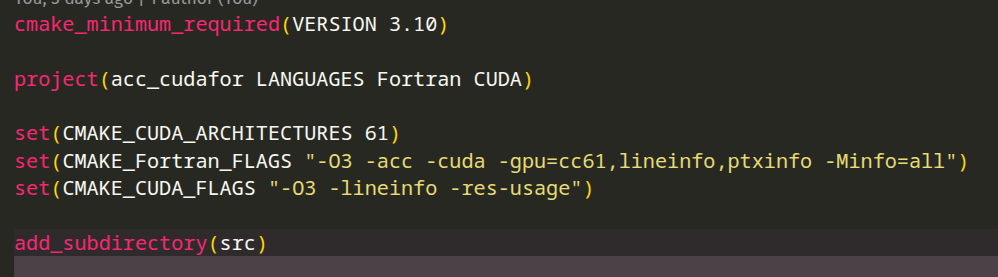
\includegraphics[width=0.99\textwidth]{images/cmakelists_1.png}
		\end{figure}
	\end{columns}
\end{frame}

\begin{frame}
	\frametitle{Example 1: ACC to CUDA}
	\begin{columns}
		\column{0.5\textwidth}
		\begin{itemize}
			\item ACC: manage device data creation and movement
			\item CUDA: define executable kernels
			\item Key detail: use of \texttt{acc host\_data use\_device} block wrapping kernel calls
			\item After update and print, another CUDA kernel is called to demonstrate that data is still on device, and usable!
			\item cuBLAS call demonstrates interoperability with CUDA libraries
			\item Exercise: run with NSYS tool to check data movements and kernel calls
		\end{itemize}
		\column{0.5\textwidth}
		\begin{figure}
			\centering
			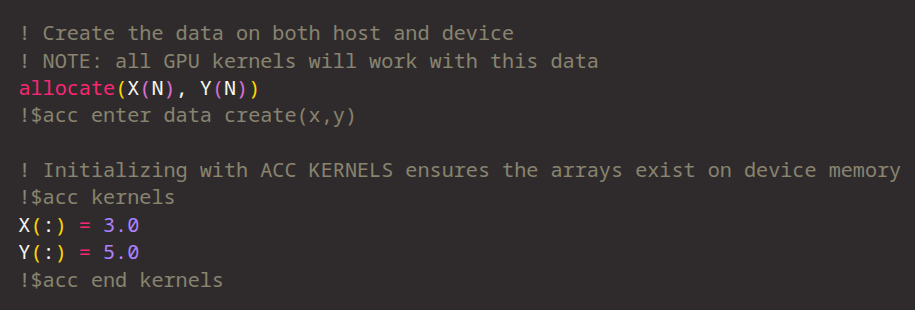
\includegraphics[width=0.9\textwidth]{images/acc2cuda_data.png}
			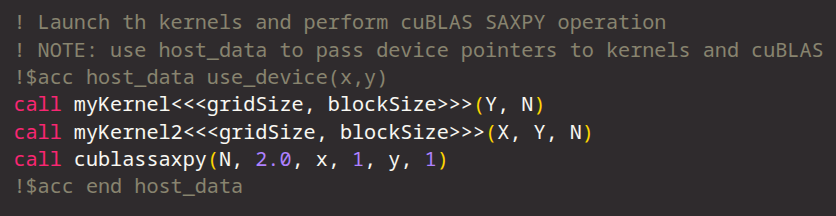
\includegraphics[width=0.9\textwidth]{images/acc2cuda_kernels.png}
		\end{figure}
	\end{columns}
\end{frame}

\begin{frame}
	\frametitle{Example 2: CUDA to ACC}
	\begin{columns}
		\column{0.5\textwidth}
		\begin{itemize}
			\item CUDA: handle device data creation and movement
			\item ACC: GPU kernels
			\item Key detail: CUDA Fortran arrays declared with \texttt{device} attribute are allocated on device (mask for \texttt{cudaMalloc})
			\item The fortran assignment operator (=) is overloaded to perform host/device copies (mask for \texttt{cudaMemcpy})
			\item ACC kernels include a subroutine call to demonstrate how a CUDA Fortran device array can be passed to an extrnal ACC kernel
			\item Exercise: run with NSYS tool to check data movements and kernel calls
		\end{itemize}
		\column{0.5\textwidth}
		\begin{figure}
			\centering
			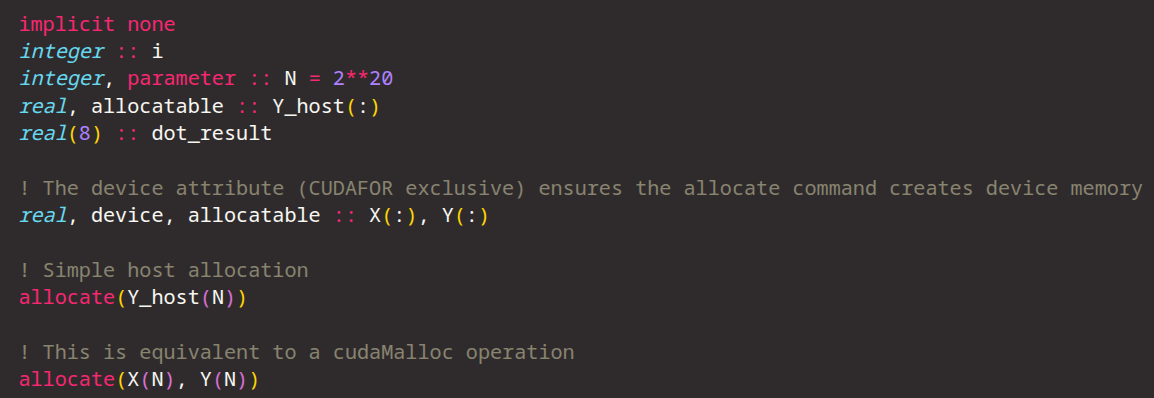
\includegraphics[width=0.9\textwidth]{images/cuda2acc_data.png}
			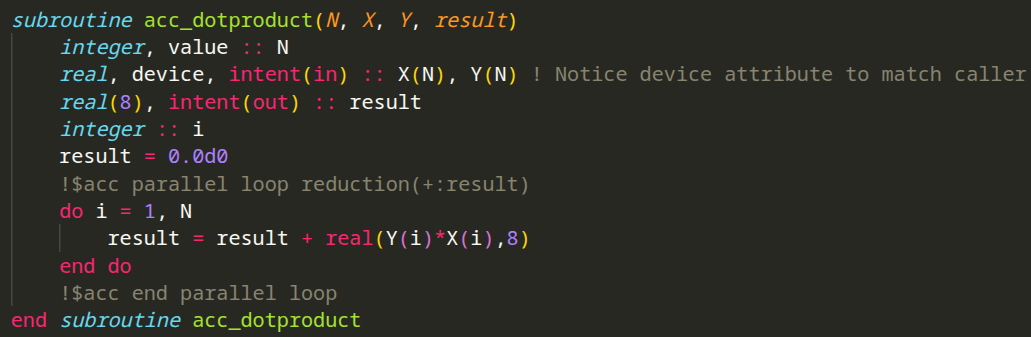
\includegraphics[width=0.9\textwidth]{images/cuda2acc_routine.png}
		\end{figure}
	\end{columns}
\end{frame}
\section{OpenACC Object Orientation}

\begin{frame}
	\frametitle{What IS an object?}
    \begin{columns}
        \column{0.5\textwidth}
            \begin{block}{Main aspects of OOP}
                \begin{itemize}
                    \item Objects: data structures containing "base" data and methods
                    \item In memory: contiguous blocks of non-static data + padding
                    \item Principles:
                    \begin{itemize}
                        \item Encapsulation: only class methods should access data
                        \item Inheritance: an object class may be derived from another
                        \item Polymorphism: methods may be redefined in derived classes
                        \item Abstraction: implementation details hidden from user
                    \end{itemize}
                \end{itemize}
            \end{block}
        \column{0.5\textwidth}
        \begin{figure}
            \centering
            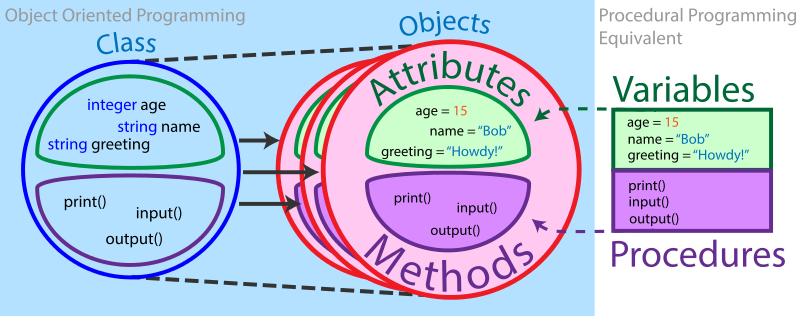
\includegraphics[width=0.95\textwidth]{images/oop.png}
            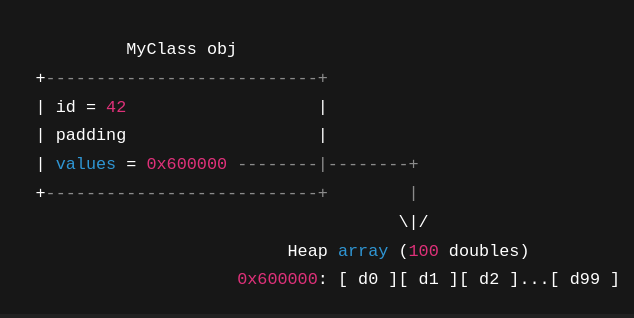
\includegraphics[width=0.95\textwidth]{images/objectLayout.png}
        \end{figure}
    \end{columns}
\end{frame}

\begin{frame}
	\frametitle{Benefits and caveats}
    \begin{columns}
        \column{0.5\textwidth}
            \begin{block}{Pros}
                \begin{itemize}
                    \item Classes are easy to reuse
                    \item Encapsulation ensures data integrity
                    \item Inheritance allows code generalization
                    \item Polymorphism allows flexible code
                    \item Abstraction allows hiding complexity
                    \item Helps to reduce function signature complexity
                    \item Design patterns + OOP can lead to VERY flexible/extensible code
                \end{itemize}
            \end{block}
        \column{0.5\textwidth}
            \begin{alertblock}{Cons}
                \begin{itemize}
                    \item Encapsulation means a LOT of extra methods...
                    \item Padding for alignment leads to memory waste
                    \item Constructor/Destructor methods require careful consideration about object lifetime
                    \item Fortran support for OOP is limited
                    \item Design patterns + OOP can lead to VERY complex code
                    \item CUDA/OpenACC not REALLY designed for OOP!
                \end{itemize}
            \end{alertblock}
    \end{columns}
\end{frame}

\begin{frame}
    \frametitle{Defining a class}
        \begin{block}{C++}
            \lstinputlisting[style=cppstyle]{../oop_disassembly/MyClass.h}
        \end{block}
\end{frame}

\begin{frame}
        \begin{block}{Fortran}
            \lstinputlisting[style=fortranstyle]{../oop_disassembly/mod_myclass.F90}
        \end{block}
\end{frame}

\begin{frame}
    \frametitle{Why OOP is tricky with ACC?}
    \begin{alertblock}{Addressing shenanigans}
        \begin{itemize}
            \item CUDA designed with C in mind: ACC follows that philosophy
            \item Objects are simple "memory blocks", containing data and pointer addresses
            \item Dynamic object data need to be created separately on the device!!!
            \item Arrays of Objects require separate allocation PER OBJECT
            \item Self instantiation on device is "possible", even for AOOs, but tricky
            \item Nested objects are possible, but VERY tricky, especially for AOOs (better with self instantiation)
            \item Fortran has VERY LIMITED support for OOP + ACC: no type-bound procedures on device, no nested AOOs!
            \item Dummy "objects" in Fortran generate copies, and may result in dangling references!
        \end{itemize}
    \end{alertblock}
\end{frame}

\begin{frame}
	\frametitle{Examples}
    \begin{itemize}
        \item Path: \texttt{Lucas/object\_oriented\_acc}
        \item Examples in both C/C++ and Fortran
        \item CMake infra for building provided for all examples
        \item Every example has a \texttt{README.md} with details and suggested exercises
        \item NOTE: some examples are intentionally flawed, as the point is to illustrate pitfalls/limitations
        \item for all examples, run with NSYS to verify memory transfers occuring (vary data sizes to see effects)
    \end{itemize}
\end{frame}

\begin{frame}
    \frametitle{Example 1: Simple objects}
    \begin{itemize}
        \item Objective: show basic object definition and usage with OpenACC
        \item Class contains a scalar and a dynamic array
        \item Fortran case: \texttt{single\_ddt\_with\_allocatable}
        \item C++ case: \texttt{struct\_with\_dynamic\_array}
        \item Key detail: it is NOT sufficient to create the object on device; dynamic data must be created separately!
        \item exercise: on the \texttt{copyout} directive, try reversing the order in which data is copied back to host. What happens?
    \end{itemize}
\end{frame}

\begin{frame}
    \frametitle{Example 2: Arrays of Structures}
    \begin{itemize}
        \item Objective: show how to handle arrays of structures with OpenACC
        \item Not quite an AOO: attributes are public, no need for getters/setters
        \item The \texttt{struct} contains a scalar and a dynamic array
        \item Fortran case: \texttt{multiple\_ddts\_with\_allocatable}
        \item C++ case: \texttt{aos\_with\_dynamic\_arrays}
        \item Key detail: now the driver allocates an array of objects, each object requiring separate allocation of its dynamic data on both host AND device!
        \item NOTE: the Fortran and C++ cases diverge a bit: in the C++ case, the host is created fully, then copied. In Fortran, the allocation loop handles both host and device sides!
        \item Exercise: in either case, the AOO + dynamic array can be substituted by a single 2D array. Try implementing this change and compare performance
    \end{itemize}
\end{frame}

\begin{frame}
    \frametitle{Example 4: Nested AOOs}
    \begin{columns}
        \column{0.5\textwidth}
            \begin{itemize}
                \item Objective: show how to handle nested AOOs with OpenACC, and imposed limitations in Fortran
                \item Russian doll of data: a root AOO where each entry contains another AOO, which in turn contains a dynamic array...
                \item Could easily occur in a FEM code: a 3D element contains an array of 2D faces, each face containing an array of 1D edges, each edge containing an array of nodes, each node containing an array of data...
                \item Allocation sizes per entry need NOT be uniform! Leads to alignment issues and other evils...
            \end{itemize}
        \column{0.5\textwidth}
            \begin{figure}
                \centering
                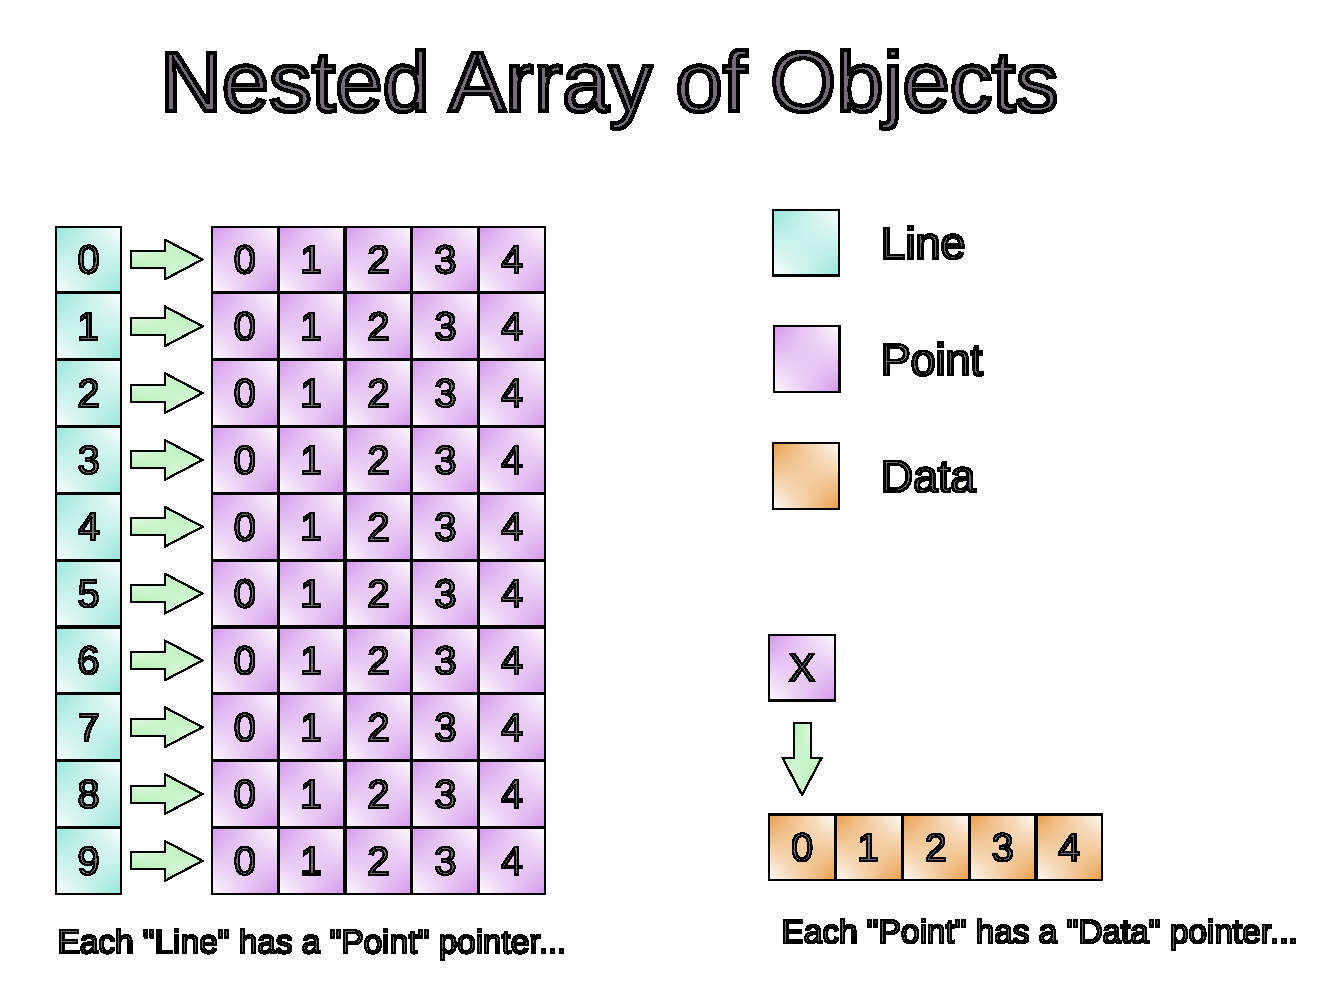
\includegraphics[width=0.95\textwidth]{images/AOO_layout.pdf}
            \end{figure}
    \end{columns}
\end{frame}

\begin{frame}
    \begin{itemize}
        \item Exercise: redo the data structures using flattened arrays (like a traditional C/Fortran code) instead of AOOs. Compare complexity and performance
    \end{itemize}
\end{frame}
\section{Closing thoughts}

\begin{frame}
    \frametitle{Conclusions: accuracy and robustness}
    \begin{itemize}
        \item Compressible TGV validation demonstrates SEM-ENVIT model to be a low-dissipation TVD scheme
        \item Both the Explicit and IMEX schemes have shown excellent converge to the reference solution
        \item Entropy viscosity has been shown to work as intended, stabilizing discontinuities without smearing turbulent structures
        \item Explicit scheme suffers from limited CFL condition on supersonic cases, further justifying the IMEX scheme
        \item Cylinder and CRM-HL demonstrate SOD2D's capability to simulate complex geometries and complex flows, demonstrate need for IMEX
    \end{itemize}
\end{frame}

\begin{frame}
    \frametitle{Conclusions: overall performance}
    \begin{itemize}
        \item Kernels have been shown to be efficient on GPUs for high-order elements
        \item Explicit vs. IMEX: dependent on the CFL limit and PCG behaviour, assuming both stable
        \item Impact of system hardware on performance has been demonstrated
        \item Importance of FP32 arithmetics usage on GPUs addressed
        \item SOD2D scalability has been demonstrated on a series of important systems
        \item Importance of proper RDMA capability in modern systems made clear
        \item SOD2D + MN5 ACC is an excellent pairing for high-performance simulations
    \end{itemize}
\end{frame}

\begin{frame}
    \frametitle{Future work}
    \begin{itemize}
        \item Test different time schemes: LS-RK and implicit variations (DIRK, ESDIRK...)
        \item Test communication strategies in MN5, as well as benefits of NCCL library usage
        \item Introduction of combustion models and chemical reactions
        \item Explore possibility of using SEM tetrahedral elements
        \item Allow for non-conformal meshes aiming at AMR
    \end{itemize}
\end{frame}

\begin{frame}
  \begin{figure}
    \centering
    
\includegraphics[width=0.7\textwidth]{images/looney.jpg}
  \end{figure}
\end{frame}

\bibliographystyle{plainnat}
\bibliography{references}

%---------------------------------------------------------

\end{document}